\chapter{Iterazione vs Ricorsione}

Spesso si confonde un \textit{costrutto linguistico} con il corrispondente \textit{processo computazionale} sottostante.

L'obiettivo è concentrarsi sul \textbf{modello computazione} indipendentemente dalla sintassi, dal linguaggio e dal costrutto linguistico usati.

\subsection{Processi computazionali iterativi}
Nei linguaggi imperativi, il costrutto linguistico che esprime un processo computazionale iterativo è tipicamente il \textbf{ciclio}.

Al di la della sintassi, esistono caratteristiche comuni:
\begin{itemize}
    \item presente un \textbf{accumulatore}
    \item inizializzazione e modifica della variabile
    \item al termine contiene il risultato
\end{itemize}

É un processo computazionale basato sulla \textit{modifica di valori}: il nuovo valore socrascrive il precedente.

\begin{minted}[bgcolor=lightgray,framesep=2mm,baselinestretch=1.2,fontsize=\footnotesize,escapeinside=||,mathescape=true]{c}
int fact = 1;

for (int i = 1; i <= n; i++) {
    fact = fact * i;
}
\end{minted}
\begin{figure}[H]
    \centering
    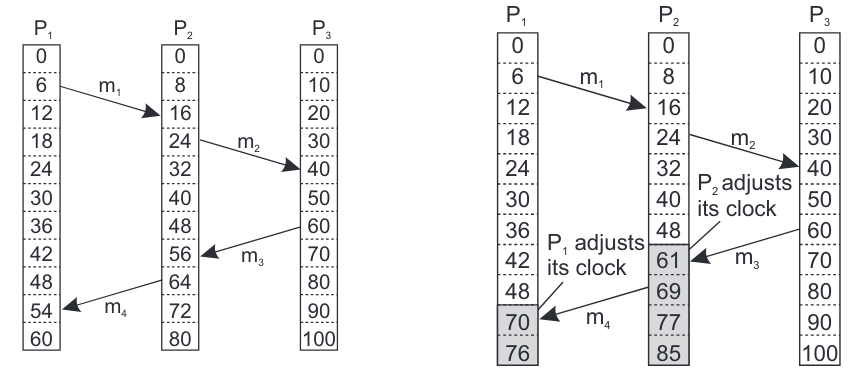
\includegraphics[width=0.4\textwidth]{/home/riccardoob/appunti/linguaggi/images/53.png}
\end{figure}

\subsection{Processi computazionali ricorsivi}
Un processo computazione \textbf{ricorsivo} è espresso da una \textit{funzione ricorsiva}.

Al di la della sintassi, esistono caratteristiche comuni:
\begin{itemize}
    \item non c'è alcun accumulatore
    \item la chiamata ricorsiva ottiene il risultato (n-1)-esimo
    \item il corpo della funzione opera sul risultato (n-1)-esimo per sintetizzare il risultato (n)-esimo desiderato
\end{itemize}

Durante le chiamate ricorsive non c'è alcun risultato parziale: si svolge solo il problema.

Il risultato è sintetizzato mentre le chiamate si \textit{chiudono}, ovvero all'indietro.

Questo è un processo computazionale basato sulla \textit{sintesi di nuovi valori} che non sovrascrivono i precedenti.

\begin{minted}[bgcolor=lightgray,framesep=2mm,baselinestretch=1.2,fontsize=\footnotesize,escapeinside=||,mathescape=true]{c}
int fact(int n) {
    return n == 0 ? 1  : fact(n - 1) * n;
}
\end{minted}
\begin{figure}[H]
    \centering
    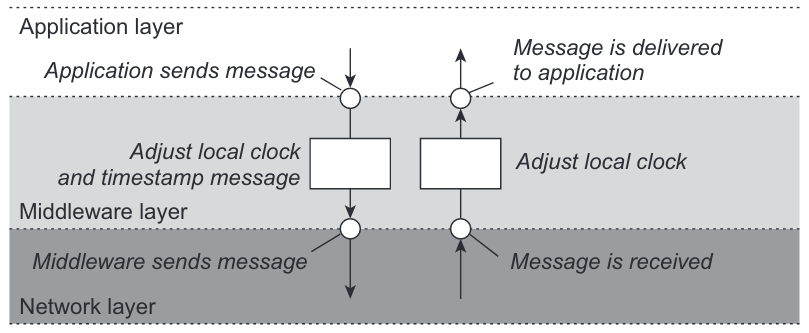
\includegraphics[width=0.6\textwidth]{/home/riccardoob/appunti/linguaggi/images/54.png}
\end{figure}

\subsection{Processi computazionali iterativi espressi da costrutti ricorsivi}
Non è sempre detto che una sintassi ricorsiva, dia luogo a un processo computazionale ricorsivo.

Un costrutto \textit{sintatticamente e formalmente ricorsivo} può dare luogo a un \textit{processo computazionale iterativo}, cioè che computa in avanti.

Ciò accade quanto la chiamata ricorsiva è l'\textit{ultima istruzione della funzione} e il risultato parziale k-esimo viene \textit{passato in avanti come argomento}.

\begin{minted}[bgcolor=lightgray,framesep=2mm,baselinestretch=1.2,fontsize=\footnotesize,escapeinside=||,mathescape=true]{c}
int factIt(int acc, int n) {
    return n == 0 ? acc : factIt(n * acc, n - 1)
}
\end{minted}

Come nel caso di un ciclo, al passo \textit{k}, l'accumulatore contiene il risultato \textit{k-esimo}.

É un processo computazionale basato sulla sintesi di \textit{nuovi valori} che però possono sovrascrivere il precedenti.

Questa è la \textbf{ricorsione in coda} (tail recursion), è un costrutto sintatticamente ricorsivo ma computazionalmente iterativo.

I linguaggi funzionali e logici tendono a usare questa ricorsione al posto dei cicli, al contrario dei linguaggi imperativi.

\subsubsection{Tail Recursion Optimization}
La tail recursion, può essere ottimizzata, stabilendo di allocare il nuovo record di attivazione sopra il precedente.

In questo modo l'occupazione delle risorse è identica a quella del ciclo.

Nei linguaggi imperativi tradizionali (C, Java, C#), la tail recursion \textit{non è ottimizzata}, in quanto sono linguaggi che offrono già una sintassi specifica per l'iterazione.

Nei linguaggi logici (Prolog) e funzionali (Lisp, Scheme) è sempre presente un sistema di TRO, così come in nuovi linguaggi \textit{blended} (Scala, Kotlin).










































